\documentclass[12pt]{article}
\usepackage{sbc-template}
%  \usepackage{subfigure}
%\usepackage{graphicx,url}
\usepackage[utf8]{inputenc}
\usepackage[brazil]{babel}
\usepackage{rotating}
\usepackage{type1ec}

%  \usepackage{subfigure}
\usepackage{chngcntr}
% \usepackage{subcaption}
\usepackage[a4paper]{geometry}
\geometry{top=3 cm,bottom=3cm,left=2.5cm,right=3cm}

% \usepackage[font=small]{caption}
%\usepackage[brazil]{babel}   
%\usepackage[latin1]{inputenc}  
%\usepackage{color}
%\usepackage[usenames,dvipsnames, table]{xcolor}
\usepackage{listings}
\usepackage{setspace}

% \usepackage{caption}   
% \captionsetup[figure]{labelsep=endash,labelfont=bf,textfont=bf}
% \captionsetup[table]{labelsep=endash,labelfont=bf,textfont=bf}
%\usepackage[most]{tcolorbox}

% Números das páginas em algarismos romanos
\pagenumbering{arabic}
\usepackage{lipsum}
\newcommand{\aspas}[1]{{``#1''}}
\newcommand{\aspassimples}[1]{{`#1'}}
\usepackage{enumerate}
\usepackage{hyperref}
\usepackage{booktabs}
\usepackage{soul}
\usepackage{setspace}
\usepackage{graphicx}
\usepackage{scrextend}
\usepackage{makeidx}
\usepackage{tabularx} % nice to have
\usepackage{array}


% % Muda as margens
% \addtolength{\oddsidemargin}{-.875in}
% 	\addtolength{\evensidemargin}{-.875in}
% 	\addtolength{\textwidth}{1.75in}

% 	\addtolength{\topmargin}{-.875in}
% 	\addtolength{\textheight}{1.75in}

\usepackage{float}
\usepackage{bm}
\usepackage{booktabs} % necessary for style
\usepackage{setspace}
\usepackage{fancy-listings}
\usepackage{colortbl}
\usepackage[table]{xcolor}  
\usepackage{adjustbox}
\usepackage{tabularx}
\usepackage{graphicx}
\usepackage{multirow}
%\newcommand{\mcode}[1]{$\mathtt{#1}$}
\newcommand*{\mcode}[1]{%
$\mathtt{#1}$%
}
%\newcommand{\mcode}[1]{\texttt{#1}}

\onehalfspacing
\setlength{\emergencystretch}{3em}
\urlstyle{rm}

%\title{Um Processo de Conformidade Arquitetural voltado à Arquitetura de Microsserviços}
\title{\textcolor{blue}{Conciliation Bank Application}:\\{\large \textcolor{blue}{Check the communication and structural design conformance}}}
%(Empresa Equals)}
%\title{ Resultado da aplicação da ferramenta DCL$^+$ na Empresa Equals}

% \author{Elena A. Araujo, Álvaro Espíndola and Ricardo}
% %{Elena A. Araujo, Ricardo Terra}

% \address{Universidade Federal de Lavras, Lavras, Brasil 
% \email{elena.araujo@posgrad.ufla.br}
% }


\definecolor{bostonuniversityred}{rgb}{0.8, 0.0, 0.0}
\definecolor{blue(pigment)}{rgb}{0.2, 0.2, 0.6}
\definecolor{verdeescuro}{rgb}{0.0, 0.44, 0.0}
\renewcommand{\lstlistingname}{Listagem}
\lstdefinestyle{colorido}{
        numbers=left,
        numberstyle=\tiny, 
        stepnumber=1,
        numberfirstline=auto,
        firstnumber=auto,
        captionpos=b,
        xleftmargin=0.4cm,
        xrightmargin=0.0cm,
        framexbottommargin=0cm,
        framextopmargin=0cm,
        boxpos=c,
        frame=single,
	    basicstyle=\linespread{0.85}\ttfamily \scriptsize,
        commentstyle=\itshape\color{darkgreen},
        showstringspaces=true,  
        mathescape=true,
        tabsize=4,
        showstringspaces=true,
        moredelim=**[is][\color{bostonuniversityred}\normalfont\bfseries]{@}{@},
        moredelim=**[is][\normalfont\bfseries\color{blue(pigment)}]{|}{|},
    moredelim=**[is][\normalfont\color{verdeescuro}]{&}{&},
    emph={[2](a), (b), (c)},emphstyle={[2]\itshape\color{gray}},
	emph={[1]only,can,cannot,depend,create,access,must,implement,useannotation,communicate, must-communicate, cannot-communicate, can-communicate, module,declare,can-communicate-only, can-depend, can-useannotation, can-throw, can-access-only, can-depend-only, cannot-depend, must-useannotation, cannot-access, must-access,must-implement, can-access, must-depend, must-extend},emphstyle={[1]\bfseries}% 	emph={Ms1_url, Ms1_repositorio, Ms1_linguagem, MsN_url, MsN_repositorio, MsN_linguagem},emphstyle={\bfseries},
%xleftmargin=0.3cm,
%xrightmargin=0.3cm,
}
\onehalfspacing



\begin{document} 
\sloppy
\maketitle

\vspace{-0.3cm}
\noindent\textbf{\large{\textcolor{blue}{Architectural design of the microservices Bank's Cconciliation application}}}
\label{sec:Estruturaltodos}

%--------------------------------------------
---------------------------


\noindent\textbf{\textcolor{blue}{\mcode{{Node}{-}{Middle}} system}}
\label{sec:ApendiceAudit}

\label{apend:especArquiteturalNodeMiddle}

%--------------------------------------------
\begin{lstlisting}[style=colorido, caption={Especificação do Projeto Arquitetural do orquestrador Node-Middle.},label={list:especArquiteturalNodeMiddle}
]
module AccessProfile: node-middleware.src.conciliacaoBancaria.accessProfile.**
module App: node-middleware.src.conciliacaoBancaria.app
module Assignment: node-middleware.src.conciliacaoBancaria.assignment.**
module AttributesSet: node-middleware.src.conciliacaoBancaria.attributesSet.**
module AuditLog: node-middleware.src.conciliacaoBancaria.auditLog.**
module BankAccounts: node-middleware.src.conciliacaoBancaria.bankAccounts.**
module BankStatement: node-middleware.src.conciliacaoBancaria.bankStatement.**
module Categories: node-middleware.src.conciliacaoBancaria.categories.**
module Cities: node-middleware.src.conciliacaoBancaria.cities.**
module Client: node-middleware.src.conciliacaoBancaria.client.**
module ConcilPlan: node-middleware.src.conciliacaoBancaria.conciliationPlan.**
module ConcilReport: node-middleware.src.conciliacaoBancaria.conciliationReport.**
module ConcilSummary: node-middleware.src.conciliacaoBancaria.conciliationSummary.**
module Config: node-middleware.src.config.**
module Dashboard: node-middleware.src.conciliacaoBancaria.dashboard.**
module Establishment: node-middleware.src.conciliacaoBancaria.establishment.**
module EstablishGroups: node-middleware.src.conciliacaoBancaria.establishmentGroups.**
module FileUpload: node-middleware.src.conciliacaoBancaria.fileUpload.**
module FinancMovements: node-middleware.src.conciliacaoBancaria.financialMovements.**
module Home: node-middleware.src.conciliacaoBancaria.home.**
module Index: node-middleware.src.conciliacaoBancaria.index
module ManualConcil: node-middleware.src.conciliacaoBancaria.manualConciliation.**
module Node_module: node-middleware.node_modules.**
module OccurrenceReason: node-middleware.src.conciliacaoBancaria.occurrenceReason.**
module OccurrenceReport: node-middleware.src.conciliacaoBancaria.occurrenceReport.**
module Operator: node-middleware.src.conciliacaoBancaria.operator.**
module ProcessedFiles: node-middleware.src.conciliacaoBancaria.processedFiles.**
module Routes: node-middleware.src.conciliacaoBancaria.routes
module States: node-middleware.src.conciliacaoBancaria.states.**
module Task: node-middleware.src.conciliacaoBancaria.task.**
module TransfData: node-middleware.src.transformationData.**
module Treegrid: node-middleware.src.conciliacaoBancaria.treegrid.**
module User: node-middleware.src.conciliacaoBancaria.user.**
#Restricoes do Projeto Arquitetural RP's
#Restricoes only-can
only App can-access Routes 																																																							"#RP1"

#Restricoes can-only
Index can-access-only App, Node_module, Config, TransfData 																							"#RP2"
App can-access-only Routes, Node_module, Config, TransfData																							"#RP3"
Routes can-access-only ConciliacaoBancaria, Node_module, Config, TransfData							"#RP4"
AccessProfile can-access-only AccessProfile, Node_module, Config, TransfData						"#RP5"
Assignment can-access-only Assignment, Node_module, Config, TransfData												"#RP6"
AttributesSet can-access-only AttributesSet, Node_module, Config, TransfData						"#RP7"
AuditLog can-access-only AuditLog, Node_module, Config, TransfData																"#RP8"@*@
BankAccounts can-access-only BankAccounts, Node_module, Config, TransfData								"#RP9"
BankStatement can-access-only BankStatement, Node_module, Config, TransfData						"#RP10"@*@
Categories can-access-only Categories, Node_module, Config, TransfData												"#RP11"
Cities can-access-only Cities, Node_module, Config, TransfData																				"#RP12"
Client can-access-only Client, Node_module, Config, TransfData																				"#RP13"
ConcilPlan can-access-only ConcilPlan, Node_module, Config, TransfData												"#RP14"
ConcilReport can-access-only ConcilReport, Node_module, Config, TransfData								"#RP15"@*@
ConcilSummary can-access-only ConcilSummary, Node_module, Config, TransfData						"#RP16"@*@
Dashboard can-access-only Dashboard, Node_module, Config, TransfData														"#RP17"@*@
Establishment can-access-only Establishment, Node_module, Config, TransfData						"#RP18"
EstablishGroups can-access-only EstablishGroups, Node_module, Config, TransfData		"#RP19"
FileUpload can-access-only FileUpload, Node_module, Config, TransfData												"#RP20"
FinancMovements can-access-only FinancMovements, Node_module, Config, TransfData		"#RP21"@*@
Home can-access-only Home, Node_module, Config, TransfData																								"#RP22"
ManualConcil can-access-only ManualConcil, Node_module, Config, TransfData								"#RP23"@*@
OccurrenceReason can-access-only OccurrenceReason, Node_module, Config, TransfData"#RP24"
OccurrenceReport can-access-only OccurrenceReport, Node_module, Config, TransfData"#RP25"@*@
Operator can-access-only Operator, Node_module, Config, TransfData																"#RP26"@*@
ProcessedFiles can-access-only ProcessedFiles, Node_module, Config, TransfData				"#RP27"
States can-access-only States, Node_module, Config, TransfData																				"#RP28"
Task can-access-only Task, Node_module, Config, TransfData																								"#RP29"
Treegrid can-access-only Treegrid, Node_module, Config, TransfData																"#RP30"
User can-access-only User, Node_module, Config, TransfData																								"#RP31"
TransfData can-access-only TransfData, Node_module, Config																								"#RP33"

#Restricoes must
Index must-access App																																																													"#RP34"
App must-access Routes																																																												"#RP35"

#Restricoes cannot
App cannot-depend Index																																																											"#RP36"
Routes cannot-depend Index, App																																																			"#RP37"

\end{lstlisting}
%--------------------------------------------
%--------------------------------------------
\begin{figure}[!ht]
\centering
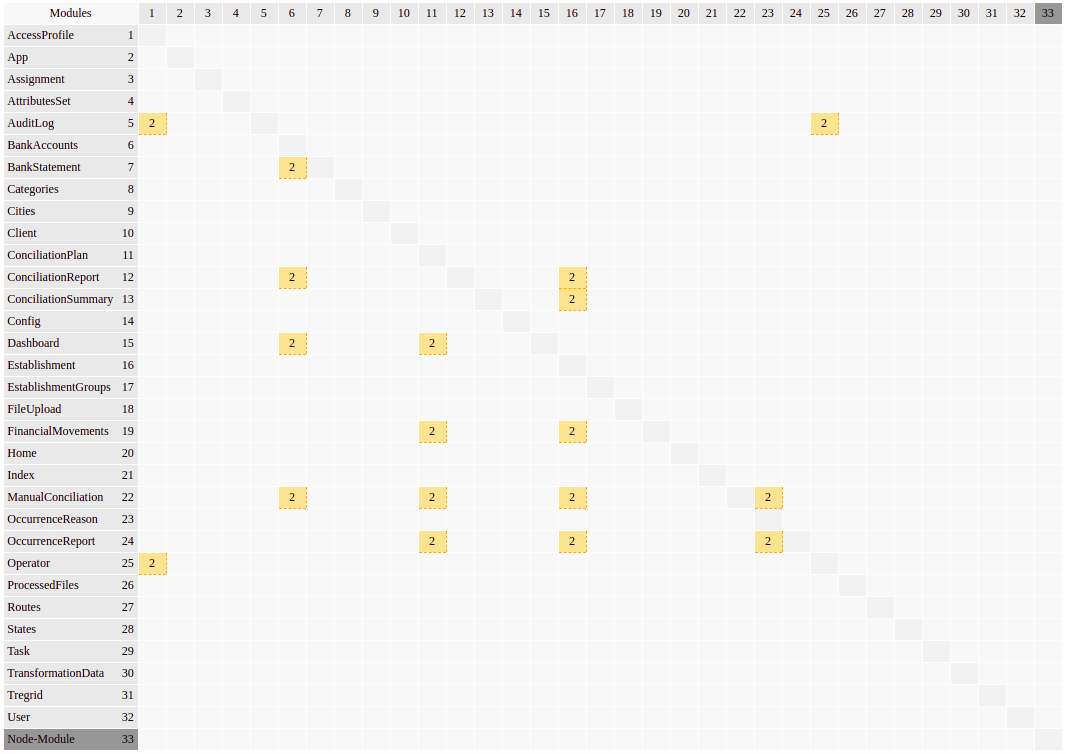
\includegraphics[width=0.99\textwidth]{figuras/violacoesNodeMiddle.png}
\vspace{-0.4cm}
\caption{\color{black}{{\mcode{{Node}}{-}\mcode{{Middle}}} architectural design violations.}}
\label{fig:violacoesNodeMiddle}
\end{figure}
%----------------

%--------------------------------------------
\noindent\textbf{\textcolor{blue}{Audit microservice}}
\label{sec:ApendiceAudit}

\vspace{-0.04cm}
%-------------------------------------------
\begin{lstlisting}[style=colorido, caption={\textcolor{blue}{Audit microservice's architectural design specification.}},label={list:especArquiteturalAudit}
]
#Internal modules of the Audit microservice
module Controller: br.com.microservices.audit.controller.*
module Domain: br.com.microservices.audit.domain.*
module Main: br.com.microservices.audit.AuditApplication
module Service: br.com.microservices.audit.services.[a-zA-Z]*Impl

#External modules of the audit microservice
module CtlrAnnotations:  org.springframework.web.bind.annotation.RequestMapping,  org.springframework.web.bind.annotation.RestController
module ExceptBC: br.com.inflexion.SpcInternalException
module MainAnnotations: org.springframework.boot.SpringApplication, org.springframework.boot.context.properties.EnableConfigurationProperties, org.springframework.boot.autoconfigure.SpringBootApplication, org.springframework.cloud.client.discovery.EnableDiscoveryClient
module Apache: org.apache.**
module ServiceAnnotation: org.springframework.stereotype.Service
module CBMultitenancy: br.com.basecommons.MultitenancyProperties
module JPA: javax.persistence.**
module Beans: org.springframework.context.**, org.springframework.beans.**
module Jndi: org.springframework.jndi.**

#Structural Design Constraints  SC's
#Only-can		
only Controller, Service can-depend Service	$\hspace{158pt}$"#Audit-SC1"
only Controller can-useannotation CtlrAnnotations $\hspace{130pt}$"#Audit-SC2"
only Service can-depend Jndi $\hspace{230pt}$"#Audit-SC3"
only Service can-throw ExceptBC	$\hspace{217pt}$"#Audit-SC4"

#Can-only
Main can-access-only Controller, MainAnnotations, Logger, Apache, java $\hspace{28pt}$"#Audit-SC5"@*@
#Cannot
Domain cannot-depend JPA $\hspace{249pt}$"#Audit-SC6"
Main cannot-depend CBMultitenancy $\hspace{206pt}$"#Audit-SC7"

#Must 
Service must-useannotation ServiceAnnotation $\hspace{154pt}$"#Audit-SC8"
\end{lstlisting}
%--------------------------------------------
%--------------------------------------------
\begin{figure}[ht]
\centering
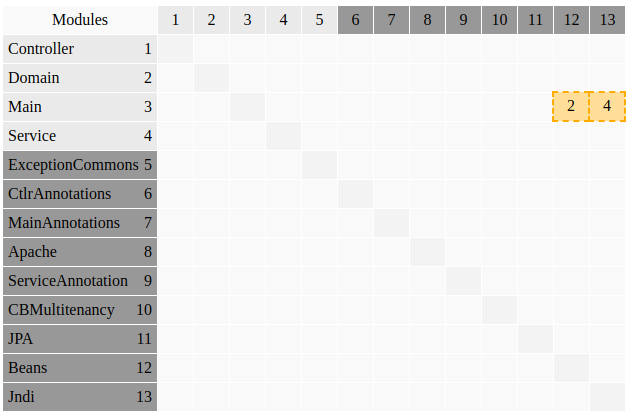
\includegraphics[width=0.6\textwidth]{figuras/violacoesAudit.png}
\caption{\textcolor{blue}{Audit microservice's architectural design violations.}}
\label{fig:microservices}
\end{figure}
%--------------------------------------------
\newpage
\noindent\textbf{\textcolor{blue}{Authentication microservice}}
\label{sec:ApendiceAuthentication}

% \vspace{-0.04cm}
%--------------------------------------------
\begin{lstlisting}[style=colorido, caption={\textcolor{blue}{Authentication microservice's architectural design specification.}},label={list:especArquiteturalAuthentication}
]
#Internal modules of the Authentication microservice
module Controller: br.com.microservices.authentication. controller.**
module Domain: br.com.microservices.authentication.domain.**
module Main: br.com.microservices.authentication.AuthenticationApplication
module Service:  br.com.microservices.authentication.service.**

#External modules
module BaseCommons:  br.com.basecommons.**
module CtlrAnnotations: org.springframework.web.bind.annotation.RequestMapping, org.springframework.web.bind.annotation.RestController
module MainAnnotations:  org.springframework.boot.SpringApplication, org.springframework.boot.context.properties.EnableConfigurationProperties, org.springframework.boot.autoconfigure.SpringBootApplication, org.springframework.cloud.client.discovery.EnableDiscoveryClient
module MyBatis: br.com.basecommons.mybatis.**
module PltDomain: br.com.plt.domain.**
module ServiceAnnotation: org.springframework.stereotype.Service

#Structural Design Constraints SC's
#Only-can
only Controller can-useannotation CtlrAnnotations $\hspace{98pt}$"#Authentication-SC1"
only Main can-useannotation MainAnnotations	$\hspace{126pt}$"#Authentication-SC2"
only Service can-useannotation ServiceAnnotation $\hspace{102pt}$"#Authentication-SC3"
only Domain, Controller, Service can-depend PltDomain $\hspace{80pt}$"#Authentication-SC4"
only Service can-depend MyBatis	$\hspace{184pt}$"#Authentication-SC5"@*@

#Cannot
system cannot-depend BaseCommons $\hspace{180pt}$"#Authentication-SC6"
Service cannot-access Controller $\hspace{180pt}$"#Authentication-SC7"

#Must
Controller must-access Service, Domain	$\hspace{151pt}$"#Authentication-SC8"
Service must-useannotation ServiceAnnotation $\hspace{122pt}$"#Authentication-SC9"@*@
Main must-useannotation MainAnnotations	$\hspace{146pt}$"#Authentication-SC10"
\end{lstlisting}
%--------------------------------------------
%--------------------------------------------
\begin{figure}[ht]
\centering
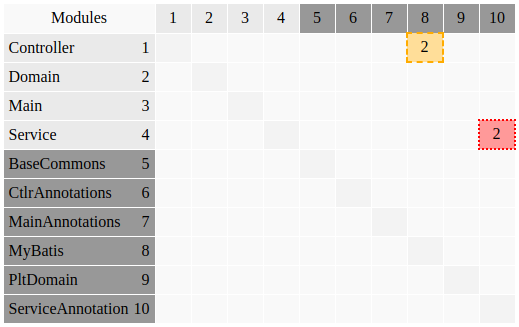
\includegraphics[width=0.65\textwidth]{figuras/violacoesAuthentication.png}
%\caption{Arquitetura de Microsserviços para o contexto de venda de produtos}
\caption{\textcolor{blue}{Authentication microservices's architectural design violations.}}
\label{fig:microservices}
\end{figure}
%--------------------------------------------
\newpage
\noindent\textbf{\textcolor{blue}{Authorization microservice}}
\label{sec:ApendiceAuthorization}
%--------------------------------------------
\begin{lstlisting}[style=colorido, caption={ \textcolor{blue}{Authorization microservice's architectural design specification.}},label={list:especArquiteturalAuthorization}
]
#Internal modules of the Authorization microservice
module Controller: br.com.microservices.authorization.controller.*
module Main: br.com.microservices.authorization.*
module ServiceInterface: br.com.microservices.authorization.services.[a-zA-Z]*Service
module ServiceImpl: br.com.microservices.authorization.services.[a-zA-Z]*Impl

#External modules
module Apache: org.apache.tomcat.**, org.apache.catalina.**, org.apache.logging.log4j.Logger
module BCMultitenancy: br.com.microservices. basecommons.multitenancy.**
module Beans: org.springframework.beans.**, org.springframework.context.**
module CtlrAnnotations: org.springframework.web.bind. annotation.RequestMapping, org.springframework.web.bind. annotation.RestController
module Jndi: org.springframework.jndi.**
module MainAnnotations: org.springframework.boot.context.properties.EnableConfigurationProperties, org.springframework.boot.autoconfigure.SpringBootApplication, org.springframework.cloud. client.discovery.EnableDiscoveryClient,  org.springframework.boot.SpringApplication
module ServiceAnnotation: org.springframework.stereotype.Service

#Structural Design Constraints SC's
#Only-can
only Controller, Service can-depend Service	$\hspace{129pt}$"#Authorization-SC1"
only Controller can-useannotation CtlrAnnotations $\hspace{101pt}$"#Authorization-SC2"
only Service can-depend Jndi $\hspace{201pt}$"#Authorization-SC3"
only Main can-depend MainAnnotations $\hspace{163pt}$"#Authorization-SC4"
	
#Can-only
Main can-depend-only java, MainAnnotations, Apache $\hspace{97pt}$"#Authorization-SC5"@*@

#Cannot
Controller cannot-access Main $\hspace{198pt}$"#Authorization-SC6"
system cannot-depend BCMultitenancy	$\hspace{170pt}$"#Authorization-SC7"
Service cannot-access Controller $\hspace{184pt}$"#Authorization-SC8"

#Must
ServiceImpl must-useannotation ServiceAnnotation $\hspace{106pt}$"#Authorization-SC9"
ServiceImpl must-implement ServiceInterface 	$\hspace{125pt}$"#Authorization-SC10"
Controller must-useannotation CtlrAnnotations $\hspace{120pt}$"#Authorization-SC11"
\end{lstlisting}
%--------------------------------------------
%--------------------------------------------
\begin{figure}[ht]
\centering
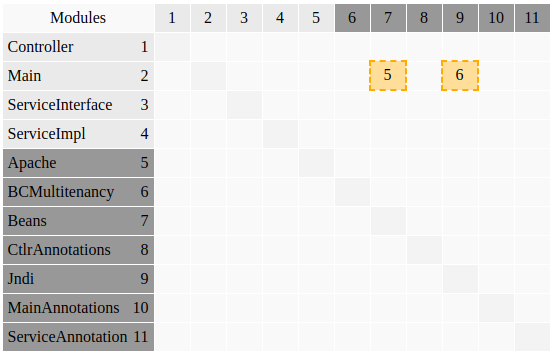
\includegraphics[width=0.75\textwidth]{figuras/violacoesAuthorization.png}
%\caption{Arquitetura de Microsserviços para o contexto de venda de produtos}
\caption{\textcolor{blue}{Authorization microservices's architectural design violations.}}
\label{fig:microservices}
\end{figure}
%--------------------------------------------

\newpage
\noindent\textbf{\textcolor{blue}{Conciliation Microservice}}
\label{sec:ApendiceConciliation}

%-------------------------------------------
\begin{lstlisting}[style=colorido, caption={\textcolor{blue}{Conciliation microservice's architectural design specification.}},label={list:especArquiteturalConciliation}
]
#Internal modules of the Conciliation microservice
module Controller: br.com.microservices.conciliation.controller.**
module DAO: br.com.microservices.conciliation.dao.**
module Domain: br.com.microservices.conciliation.domain.**
module ImplementDAO: br.com.microservices.conciliation.dao.[a-zA-Z]*DaoImpl
module Util: br.com.microservices.conciliation.util.**
module Main: br.com.microservices.conciliation.ConciliationApplication
module Service: br.com.microservices.conciliation.service.**
module Scheduled:  br.com.microservices.conciliation.scheduled.**

#External Modules
module AmazonSQS: com.amazonaws.services.sqs.AmazonSQS
module Beans: org.springframework.beans.**, org.springframework.stereotype.Component
module BCDAO: br.com.basecommons.daos.**
module BCDomain: br.com.basecommons.domain.*
module BCModel: br.com.basecommons.models.*
module BCMultitenancy: br.com.basecommons.multitenancy.**
module CtlrAnnotations: org.springframework.web.bind.annotation.RequestMapping, org.springframework.web.bind.annotation.RestController
module JPA: javax.persistence.**
module Logger: org.apache.logging.log4j.Logger
module MainAnnotations: org.springframework.boot.SpringApplication org.springframework.boot.context.properties.EnableConfigurationProperties, org.springframework.boot.autoconfigure.SpringBootApplication, org.springframework.cloud.client.discovery.EnableDiscoveryClient
module ServiceAnnotation: org.springframework.stereotype.Service
module SpringRepository: org.springframework.stereotype.Repository

#Structural Design Constraints SC's
#Only-can
only Controller can-useannotation CtlrAnnotations $\hspace{106pt}$"#Conciliation-SC1"
only Scheduled can-depend AmazonSQS	$\hspace{173pt}$"#Conciliation-SC2"
only Service can-access DAO	$\hspace{212pt}$"#Conciliation-SC3"
only Controller, Service can-access Service $\hspace{135pt}$"#Conciliation-SC04"
only Main can-depend BCMultitenancy	$\hspace{174pt}$"#Conciliation-SC5"
only DAO, Service can-depend BCDAO	$\hspace{179pt}$"#Conciliation-SC6"
	
#Can-only
Util can-depend-only Util, java, Logger $\hspace{155pt}$"#Conciliation-SC7"@*@
only Scheduled can-depend AmazonSQS	 $\hspace{174pt}$"#Conciliation-SC8"
Domain can-access-only BCModel, BCDomain, java $\hspace{122pt}$"#Conciliation-SC9"
ImplementDAO can-depend-only JPA, Hibernate, java, SpringRepository, BCModel$\hspace{293pt}$"#Conciliation-SC"10
Main can-access-only Controller, MainAnnotations, Logger, java $\hspace{44pt}$"#Conciliation-SC11"

#Cannot
Domain cannot-depend JPA $\hspace{227pt}$"#Conciliation-SC12"
Controller cannot-access DAO $\hspace{208pt}$"#Conciliation-SC13"

#Must
Main must-useannotation MainAnnotation	$\hspace{160pt}$"#Conciliation-SC14"
ImplementDAO must-depend SpringRepository $\hspace{146pt}$"#Conciliation-SC15"
Service must-useannotation ServiceAnnotation $\hspace{131pt}$"#Conciliation-SC16"
\end{lstlisting}
%--------------------------------------------
%--------------------------------------------
\begin{figure}[ht]
\centering
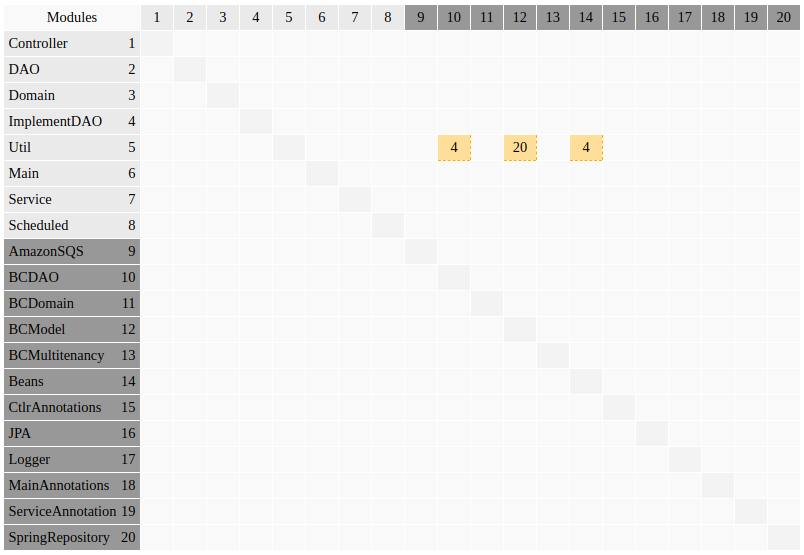
\includegraphics[width=0.75\textwidth]{figuras/violacoesConciliation.png}
%\caption{Arquitetura de Microsserviços para o contexto de venda de produtos}
\caption{\textcolor{blue}{Conciliation microservices's architectural design violations.}}
\label{fig:microservices}
\end{figure}
%--------------------------------------------

\newpage
\noindent\textbf{\large{\textcolor{blue}{Dashboard}}}
\label{sec:ApendiceDashboard}


%--------------------------------------------
\vspace{0.2cm}
\begin{lstlisting}[style=colorido, caption={\textcolor{blue}{Dashboard microservice's architectural design specification.}},label={list:especArquiteturalDashboard}
]
module Controller: br.com.microservices.dashboard.controller.*
module DAO: br.com.microservices.dashboard.dao.**
module DAOInterface: br.com.microservices.dashboard.dao.[a-zA-Z]*Dao
module Service: br.com.microservices.dashboard.service.*

#External Modules
module BCController: br.com.basecommons.controller.**
module BCModel: br.com.basecommons.models.**
module CtlrAnnotations: org.springframework.web.bind.annotation.RequestMapping, org.springframework.web.bind. annotation.RestController
module Hibernate: org.hibernate.**
module MainAnnotations: org.springframework.boot.context.properties.EnableConfigurationProperties, org.springframework.boot.autoconfigure.SpringBootApplication, org.springframework.cloud.client.discovery.EnableDiscoveryClient, org.springframework.boot.SpringApplication
module ServiceAnnotation: org.springframework.stereotype.Service
module SpringRepository: org.springframework.stereotype.Repository

#Structural Design Constraints SC's
#Only-can
only Controller can-useannotation CtlrAnnotations $\hspace{111pt}$"#Dashboard-SC1"
only Controller can-depend BCController	$\hspace{159pt}$"#Dashboard-SC2"
only Main can-depend BCMultitenancy	$\hspace{179pt}$"#Dashboard-SC3"
only Service, DAO can-access DAO $\hspace{193pt}$"#Dashboard-SC4"

#Can-only
ImplementDAO can-depend-only JPA, Hibernate, java, SpringRepository, BCModel$\hspace{297pt}$"#Dashboard-SC5"

#Cannot
Controller cannot-access DAO $\hspace{212pt}$"#Dashboard-SC6"
Service cannot-depend Controller $\hspace{193pt}$"#Dashboard-SC7"

#Must
Main must-useannotation MainAnnotations	$\hspace{158pt}$"#Dashboard-SC8"

Controller must-access Service	$\hspace{201pt}$"#Dashboard-SC9"@*@
ImplementDAO must-implement DAOInterface $\hspace{154pt}$"#Dashboard-SC10"
ImplementDAO must-depend SpringRepository $\hspace{149pt}$"#Dashboard-SC11"
Service must-useannotation ServiceAnnotation $\hspace{134pt}$"#Dashboard-SC12"
\end{lstlisting}
%--------------------------------------------
% %--------------------------------------------
% \begin{figure}[ht]
% \centering
% 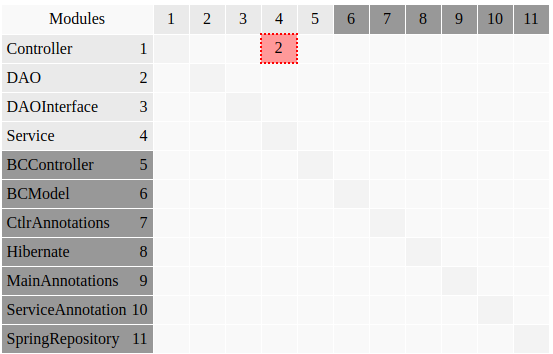
\includegraphics[width=0.7\textwidth]{figuras/violacoesDashboard.png}
% %\caption{Arquitetura de Microsserviços para o contexto de venda de produtos}
% \caption{\textcolor{blue}{Dashboard microservices's architectural project violations.}}
% \label{fig:microservices}
% \end{figure}
% %--------------------------------------------

% \newpage
\noindent\textbf{\large{\textcolor{blue}{Entries microservice}}}
\label{sec:ApendiceEntries}


%--------------------------------------------
\begin{lstlisting}[style=colorido, caption={ \textcolor{blue}{Entries microservice's architectural design specification.}},label={list:especArquiteturalEntries}
]
 #Internal modules of the Entries microservice
module Util: br.com.microservices.entries.utils.*
module Controller:  br.com.microservices.entries.controller.*
module DAO: br.com.microservices.entries.dao.*
module ImplementDAO: br.com.microservices.entries.dao. [a-zA-Z]*DaoImpl
module Main: br.com.microservices.entries.EntriesApplication
module Model: br.com.microservices.entries.model.**, br.com.microservices.entries.model.**, br.com.microservices.entries.models.**
module Service: br.com.microservices.entries.service.**
module ServiceImplement: br.com.microservices.entries.service.*[a-zA-Z]*ServiceImpl
module Serializer: br.com.microservices.entries.serializer.*

#External Modules
module BCMultitenancy: br.com.basecommons.multitenancy.**	
module CtlrAnnotations: org.springframework.web.bind. annotation.RequestMapping, org.springframework.web.bind. annotation.RestController
module Hibernate: org.hibernate.**
module JPA: javax.persistence.**
module MainAnnotations: org.springframework.boot.SpringApplication org.springframework.boot.context.properties.EnableConfigurationProperties, org.springframework.boot.autoconfigure.SpringBootApplication, org.springframework.cloud.client.discovery.EnableDiscoveryClient
module Serializable: java.io.Serializable
module ServiceAnnotation: org.springframework.stereotype.Service	
module SpringRepository: org.springframework.stereotype.Repository

#Structural Design Constraints SC's
#Only-can 
only Controller can-useannotation CtlrAnnotations $\hspace{123pt}$"#Entries-SC1"
only Controller, Service can-access Service	$\hspace{152pt}$"#Entries-SC2"
only Service can-access DAO	$\hspace{229pt}$"#Entries-SC3"
only Main can-depend BCMultitenancy $\hspace{190pt}$"#Entries-SC4"@*@

#Can-only
Util can-depend-only Util, java	$\hspace{210pt}$"#Entries-SC5"@*@
ImplementDAO can-depend-only JPA, Hibernate, SpringRepository, java	$\hspace{37pt}$"#Entries-SC6"

#Cannot
Controller cannot-access DAO $\hspace{224pt}$"#Entries-SC7"@*@

#Must
Main must-useannotation MainAnnotations	$\hspace{170pt}$"#Entries-SC8"
Controller must-useannotation CtlrAnnotations $\hspace{143pt}$"#Entries-SC9"
Service must-useannotation ServiceAnnotation $\hspace{147pt}$"#Entries-SC10"
Model, Serializer must-implement Serializable $\hspace{143pt}$"#Entries-SC11"@*@
ImplementDAO must-implement SpringRepository $\hspace{147pt}$"#Entries-SC12"

\end{lstlisting}
%--------------------------------------------
%--------------------------------------------
\begin{figure}[ht]
\centering
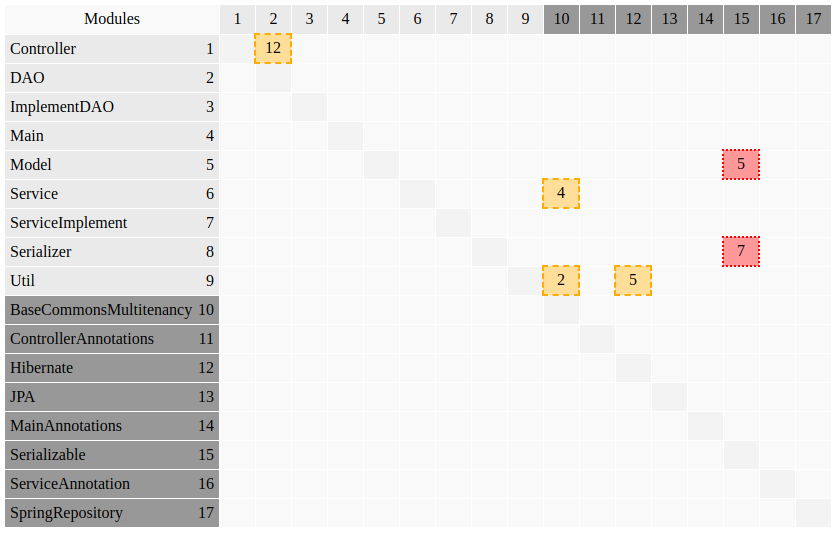
\includegraphics[width=0.7\textwidth]{figuras/violacoesEntries.png}
%\caption{Arquitetura de Microsserviços para o contexto de venda de produtos}
\caption{\textcolor{blue}{Entries microservices's architectural design violations.}}
\label{fig:microservices}
\end{figure}
%--------------------------------------------


\newpage
\noindent\textbf{\large{\textcolor{blue}{FileLoad microservice}}}
\label{sec:ApendiceFileLoad}


%--------------------------------------------
\begin{lstlisting}[style=colorido, caption={\textcolor{blue}{FileLoad microservice's architectural design specification.}},label={list:especArquiteturalFileLoad}
]
#Internal modules of the  FileLoad microservice
module DAO: br.com.microservices.fileload.daos.*
module DAOInterface: br.com.microservices.fileload.daos.[a-zA-Z]*Dao
module ImplementDAO: br.com.microservices.fileload.daos.[a-zA-Z]*DaoImpl
module Main: br.com.microservices.fileload.*
module Model: br.com.microservices.fileload.models.**
module Service: br.com.microservices.fileload.services.*

#External Modules
module BCDAO: br.com.basecommons.daos.**
module BCModel: br.com.basecommons.basecommons.models.*
module BCMultitenancy: br.com.basecommons.multitenancy.**
module Beans: javax.validation.**
module DataSource: org.springframework.boot.autoconfigure.
jdbc.DataSourceAutoConfiguration
module Hibernate: org.hibernate.**
module JPA: javax.persistence.**
module MainAnnotations: org.springframework.boot.SpringApplication, 
org.springframework.boot.context.properties.EnableConfigurationProperties, org.springframework.boot.autoconfigure.SpringBootApplication, org.springframework.cloud.client.discovery.EnableDiscoveryClient
module Serializable: java.io.Serializable
module ServiceAnnotation: org.springframework.stereotype.Service
module SpringRepository: org.springframework.stereotype.Repository

#Structural Design Constraints SC's
#Only-can 
only Model, DAO can-depend JPA, Beans $\hspace{175pt}$"#FileLoad-SC1"
only Main can-useannotation MainAnnotations, DataSource $\hspace{88pt}$"#FileLoad-SC2"
only Main can-depend BCMultitenancy	$\hspace{184pt}$"#FileLoad-SC3"
only Service can-useannotation ServiceAnnotation $\hspace{122pt}$"#FileLoad-SC4"

#Can-only
ImplementDAO can-depend-only JPA, Hibernate, BCModel, SpringRepository $\hspace{17pt}$"#FileLoad-SC5"
	
#Cannot
Main cannot-depend DAO, Model, BCDAO, JPA $\hspace{156pt}$"#FileLoad-SC6"@*@
Service cannot-access Main $\hspace{228pt}$"#FileLoad-SC7"

#Must
ImplementDAO must-implement DAOInterface $\hspace{161pt}$"#FileLoad-SC8"
ImplementDAO must-depend SpringRepository $\hspace{157pt}$"#FileLoad-SC9"
Model must-implement Serializable $\hspace{195pt}$"#FileLoad-SC10"@*@
Service must-useannotation ServiceAnnotation $\hspace{142pt}$"#FileLoad-SC11"
\end{lstlisting}
%--------------------------------------------
%--------------------------------------------
\begin{figure}[ht]
\centering
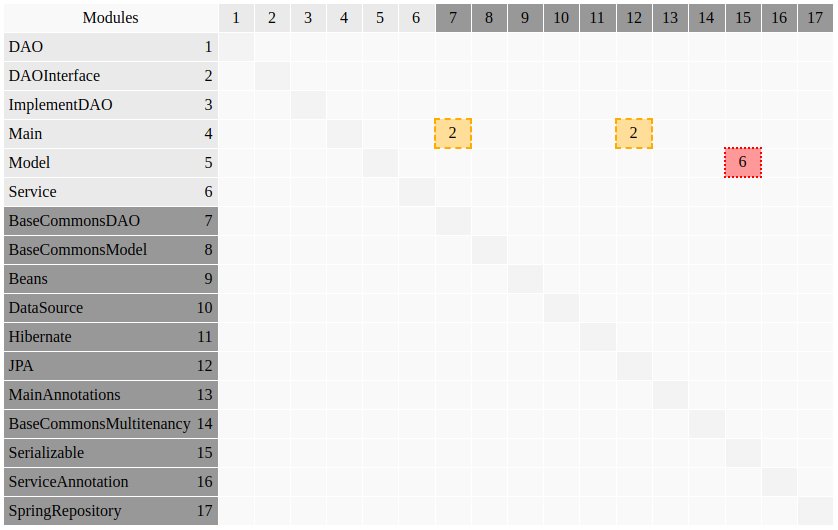
\includegraphics[width=0.7\textwidth]{figuras/violacoesFileLoad.png}
\vspace{-0.2cm}
\caption{\textcolor{blue}{FileLoad microservices's architectural design violations.}}
\label{fig:microservices}
\end{figure}
%--------------------------------------------

% \newpage
\noindent\textbf{\large{\textcolor{blue}{FileProcess microservice}}}
\label{sec:ApendiceFileProccess}


%--------------------------------------------
\begin{lstlisting}[style=colorido, caption={\textcolor{blue}{FileProcess microservice's architectural design specification.}},label={list:especArquiteturalFileProccess}
]
#Internal modules of the FileProcess microservice
module DAO: br.com.microservices.process.dao.**
module DAOInterface: br.com.microservices. process.dao.[a-zA-Z]*Dao
module ImplementDAO: br.com.microservices. process.dao.[a-zA-Z]*DaoImpl
module Main: br.com.microservices.process.Application
module Model: br.com.microservices.model.**
module Scheduling: br.com.microservices.schedule.**
module Service: br.com.microservices.service.**
module Util: br.com.microservices.process.util.**

#External Modules
module AmazonService: com.amazonaws.services.**
module BCDomain: equals.gestaofinanceira.microservices.cba. basecommons.domain.**
module BCUtil: br.com.basecommons.utils.**
module BCMultitenancy: br.com.basecommons.multitenancy.**
module JPA: javax.persistence.**
module Logger: org.apache.logging.log4j.Logger
module MainAnnotations: org.springframework.boot.SpringApplication, org.springframework.boot.context.properties.EnableConfigurationProperties, org.springframework.boot.autoconfigure.SpringBootApplication, org.springframework.cloud.client.discovery.EnableDiscoveryClient
module ScdAnnotation: org.springframework.scheduling. annotation.EnableScheduling
module ScdFramework: org.springframework.scheduling.**
module Serializable: java.io.Serializable
module ServiceAnnotation: org.springframework.stereotype.Service
module SpringBeans: org.springframework.beans.**
module SpringRepository: org.springframework.stereotype.Repository

#Structural Design Constraints SC's
#Only-can
only Main can-useannotation MainAnnotations	$\hspace{136pt}$"#FileProcess-SC1"
only Scheduling can-access ScdFramework $\hspace{155pt}$"#FileProcess-SC2"
only Main can-depend BCMultitenancy $\hspace{174pt}$"#FileProcess-SC3"
only DAO, Model can-depend JPA	$\hspace{198pt}$"#FileProcess-SC4"@*@
only Service, Scheduling can-depend AmazonService 	$\hspace{103pt}$"#FileProcess-SC5"

#Can-only
Util can-depend-only Util, BCUtil, java, Logger $\hspace{116pt}$"#FileProcess-SC6"@*@
    
#Cannot
Service cannot-depend Controller $\hspace{188pt}$"#FileProcess-SC7"
    
#Must
Main must-useannotation MainAnnotations	$\hspace{155pt}$"#FileProcess-SC8"
Service must-useannotation ServiceAnnotation $\hspace{131pt}$"#FileProcess-SC9"
ImplementDAO must-implement DAOInterface, SpringRepository $\hspace{64pt}$"#FileProcess-SC10"
Model must-implement Serializable $\hspace{184pt}$"#FileProcess-SC11"@*@
Scheduling must-depend ScdFramework $\hspace{175pt}$"#FileProcess-SC12"
Scheduling must-useannotation ScdAnnotation $\hspace{136pt}$"#FileProcess-SC13"
\end{lstlisting}

%--------------------------------------------
%--------------------------------------------
\begin{figure}[ht]
\centering
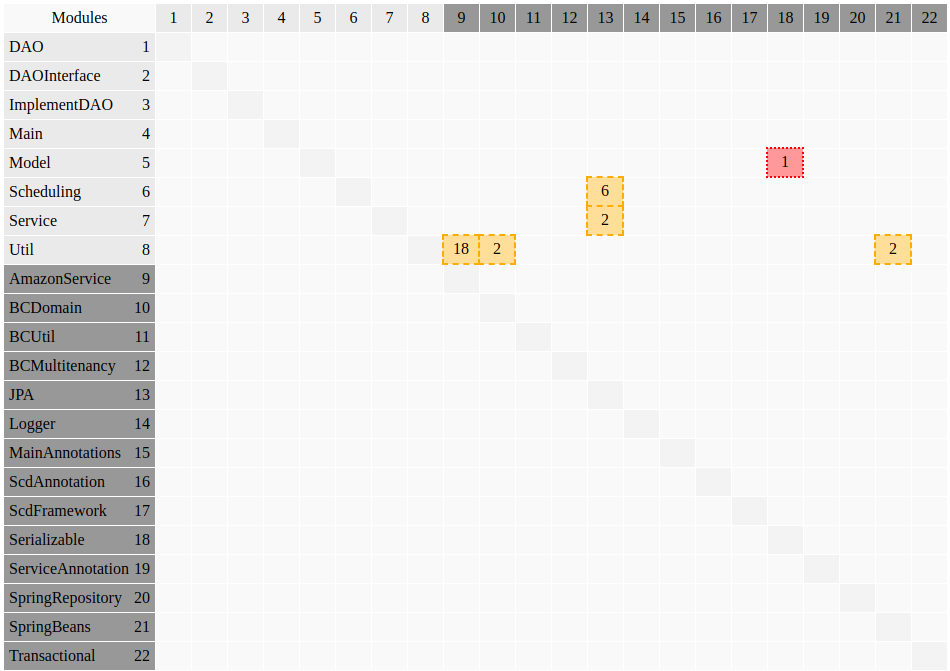
\includegraphics[width=0.75\textwidth]{figuras/violacoesFileProccess.png}
\caption{\textcolor{blue}{FileProcess microservices's architectural design violations.}}
\label{fig:microservices}
\end{figure}
%--------------------------------------------


% \newpage
\noindent\textbf{\large{\textcolor{blue}{Reports microservice}}}
\label{sec:ApendiceReports}

%--------------------------------------------
\begin{lstlisting}[style=colorido,caption={\textcolor{blue}{Reports microservice's architectural design specification.}},label={list:especArquiteturalReports}
]
#Internal modules of the Reports microservice
module Controller: br.com.microservices.reports.controller.**
module Main: br.com.microservices.reports.ReportsApplication
module Serializer: br.com.microservices.reports.serializer.**
module Service: br.com.microservices.reports.service.**

#External Modules
module BCController: br.com.basecommons.controller.BaseController
module BCMultitenancy: br.com.basecommons.basecommons.multitenancy.properties.MultitenancyProperties
module CtlrAnnotations: org.springframework.web.bind.annotation.RequestMapping, org.springframework.web.bind.annotation.RestController, ControllerAnnotations.**
module JSONSerializer: flexjson.JSONSerializer.*
module MainAnnotations: org.springframework.boot.SpringApplication,  org.springframework.boot.context.properties.EnableConfigurationProperties, org.springframework.boot.autoconfigure.SpringBootApplication, org.springframework.cloud.client.discovery.EnableDiscoveryClient
module ServiceAnnotation: org.springframework.stereotype.Service

#Structural Design Constraints SC's
#Only-can
only Controller can-useannotation CtlrAnnotations $\hspace{120pt}$"#Reports-SC1"
only Main can-depend BCMultitenancy $\hspace{187pt}$"#Reports-SC2"
only Main can-useannotation MainAnnotations $\hspace{148pt}$"#Reports-SC3"

#Cannot
Service cannot-access Controller $\hspace{202pt}$"#Reports-SC4"

#Must	
Main must-useannotation MainAnnotation  $\hspace{173pt}$"#Reports-SC5"
Controller must-useannotation CtlrAnnotations $\hspace{139pt}$"#Reports-SC6"@*@
Controller must-extend BCController	$\hspace{187pt}$"#Reports-SC7"@*@
Service must-useannotation ServiceAnnotation $\hspace{144pt}$"#Reports-SC8"
Serializer must-depend JSONSerializer	$\hspace{178pt}$"#Reports-SC9"@*@

\end{lstlisting}
%--------------------------------------------
%--------------------------------------------
\begin{figure}[ht]
\centering
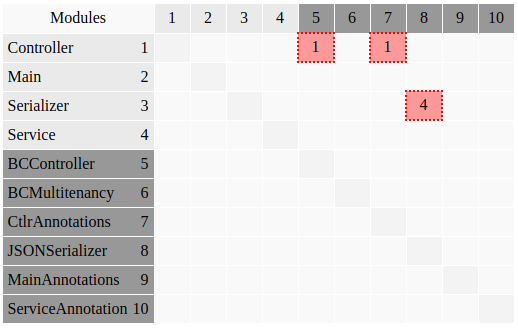
\includegraphics[width=0.65\textwidth]{figuras/violacoesReports.png}
\caption{\textcolor{blue}{Reports microservices's architectural design violations.}}
\label{fig:microservices}
\end{figure}
%--------------------------------------------

\newpage
\noindent\textbf{\large{\textcolor{blue}{Summary microservice}}}
\label{sec:ApendiceSummary}

%--------------------------------------------
\begin{lstlisting}[style=colorido, caption={\textcolor{blue}{Summary microservice's architectural design specification.}},label={list:especArquiteturalSummary}
]
#Internal modules of the Summary microservice
module BaseService:  br.com.microservices.summary.service.BaseService
module Controller:  br.com.microservices.summary.controller.*
module DAO: br.com.microservices.summary.dao.*
module DAOInterface: br.com.microservices.summary.dao.[a-zA-Z]*Dao
module ImplementDAO: br.com.microservices.summary.dao.[a-zA-Z]*Impl
module Main: br.com.microservices.summary.SummaryApplication
module Service: br.com.microservices.summary.service.*
module ServiceSubClass: br.com.microservices.summary.service.AtributoService, br.com.microservices.summary.service.ConciliacaoService, br.com.microservices.summary.service.TreegridService
module Stream: br.com.microservices.summary.stream.*
module Util: br.com.microservices.summary.util.**

#External Modules
module BCMultitenancy: br.com.basecommons.multitenacy.**
module CtlrAnnotations: org.springframework.web.bind.annotation.RequestMapping, org.springframework.web.bind. annotation.RestController
module MainAnnotations:  org.springframework.boot.SpringApplication, org.springframework.boot.context.properties.EnableConfigurationProperties, org.springframework.boot.autoconfigure.SpringBootApplication, org.springframework.cloud.client.discovery.EnableDiscoveryClient
module Repository: org.springframework.stereotype.Repository
module ServiceAnnotation: org.springframework.stereotype.Service

#Structural Design Constraints SC's
#Only-can
only Service can-useannotation ServiceAnnotation $\hspace{118pt}$"#Summary-SC1" 
only Controller can-useannotation CtlrAnnotations	$\hspace{114pt}$"#Summary-SC2"
only Main can-useannotation MainAnnotations	$\hspace{142pt}$"#Summary-SC3"
only Main can-depend BCMultitenancy $\hspace{180pt}$"#Summary-SC4"

#Can-only	
Util can-access-only Util, java $\hspace{200pt}$"#Summary-SC5"

#Must
Main must-useannotation MainAnnotations	$\hspace{162pt}$"#Summary-SC6"
Service must-useannotation ServiceAnnotation $\hspace{138pt}$"#Summary-SC7"@*@
Controller must-useannotation CtlrAnnotations $\hspace{133pt}$"#Summary-SC8"@*@
ServiceSubClass must-extend BaseService	$\hspace{163pt}$"#Summary-SC9"
ImplementDAO must-implement DAOInterface $\hspace{158pt}$"#Summary-SC10"
ImplementDAO must-useannotation Repository $\hspace{148pt}$"#Summary-SC11"
Controller must-access Stream $\hspace{210pt}$"#Summary-SC12"
\end{lstlisting}
%--------------------------------------------
%--------------------------------------------
\begin{figure}[ht]
\centering
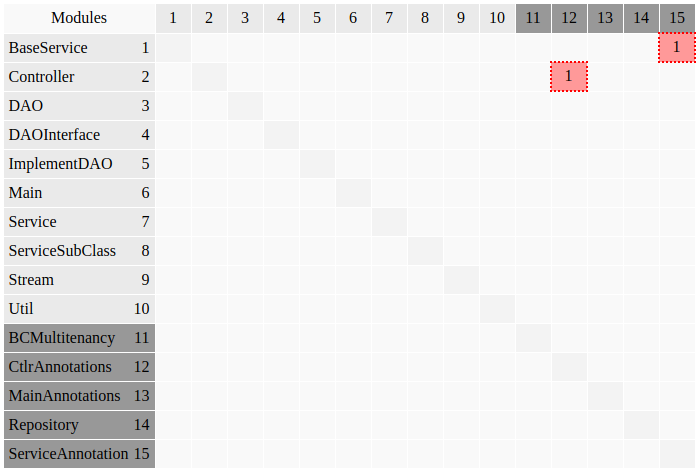
\includegraphics[width=0.7\textwidth]{figuras/violacoesSummary.png}
\caption{\textcolor{blue}{Summary microservices's archictetural design violations.}}
\label{fig:microservices}
\end{figure}
%--------------------------------------------
% 
%--------------------------------------------
% \newpage
% % Please add the following required packages to your document preamble:
% % \usepackage{multirow}
% \begin{table}[]
%   \begin{adjustbox}{width=\textwidth}

% \footnotesize
% \begin{tabular}{|l|l|l|l|l|}
% \hline
% Módulo                                                                           & Restrição                                                                                                                                                                                                         & Viol.              & Comunicação violada                                                                                                                         & Local da violação                                                                                         \\ \hline
% \multirow{3}{*}{Assigment}                                                       & \multirow{2}{*}{Assigment can-communicate-only reports}                                                                                                                                                           & \multirow{2}{*}{2} & \begin{tabular}[c]{@{}l@{}}Assigment communicates entries \\ using /cliente/\$clientId/tarefas\end{tabular}                                 & \begin{tabular}[c]{@{}l@{}}\$system/assignment/assignment.js\\ (linha …)\end{tabular}                     \\ \cline{4-5} 
%                                                                                  &                                                                                                                                                                                                                   &                    & \begin{tabular}[c]{@{}l@{}}Assigment communicate entries \\ using cliente/\$clientId/\\ tarefaTipoVinculo/\$tarefaId\end{tabular}             & \begin{tabular}[c]{@{}l@{}}\$system/assignment/assignment.js \\ (linha ..)\end{tabular}                   \\ \cline{2-5} 
%                                                                                  & Assigment must-communicate reports                                                                                                                                                                                &                    & --                                                                                                                                          & --                                                                                                        \\ \hline
% \multirow{2}{*}{\begin{tabular}[c]{@{}l@{}}Occurrence-\\ Report\end{tabular}}    & \begin{tabular}[c]{@{}l@{}}OccurrenceReport can-communicate-only \\ reports\end{tabular}                                                                                                                          & \multirow{2}{*}{1} & \begin{tabular}[c]{@{}l@{}}OccurrenceReport communicates \\ entries using /cliente/\$clientId/\\ atributos\end{tabular}                     & \begin{tabular}[c]{@{}l@{}}\$system/occurrenceReport/\\ occurrenceReport.js (linha ..)\end{tabular}       \\ \cline{2-2} \cline{4-5} 
%                                                                                  & \begin{tabular}[c]{@{}l@{}}OccurrenceReport must-communicate \\ reports\end{tabular}                                                                                                                              &                    & --                                                                                                                                          & --                                                                                                        \\ \hline
                                                                                 
% \multirow{2}{*}{\begin{tabular}[c]{@{}l@{}}Financial-\\ Movements\end{tabular}}    & \begin{tabular}[c]{@{}l@{}}FinancialMovements can-communicate-only \\ reports\end{tabular}                                                                                                                          & \multirow{2}{*}{1} & \begin{tabular}[c]{@{}l@{}}FinancialMovements communicate \\entries using /cliente/\$clientId/atributos
% \end{tabular}                     & \begin{tabular}[c]{@{}l@{}}\$system/financialMovements/\\financialMovements.js (linha …)\end{tabular}       \\ \cline{2-2} \cline{4-5} 
%                                                                                  & \begin{tabular}[c]{@{}l@{}}
% FinancialMovements must-communicate \\reports 
% \end{tabular}                                                                                                                              &                    & --                                                                                                                                          & --                                                                                                        \\ \hline
% \multirow{5}{*}{\begin{tabular}[c]{@{}l@{}}Conciliation-\\ Report\end{tabular}}  & \multirow{4}{*}{\begin{tabular}[c]{@{}l@{}}ConciliationReport can-communicate-only\\ reports\end{tabular}}                                                                                                        & \multirow{4}{*}{4} & \begin{tabular}[c]{@{}l@{}}ConciliationReport communicates \\ summary using /cliente/\$clientId/\\ detalheConciliacaoDownload\end{tabular}  & \begin{tabular}[c]{@{}l@{}}\$system//conciliationReport/\\ conciliationReport.js (linha ..)\end{tabular}  \\ \cline{4-5} 
%                                                                                  &                                                                                                                                                                                                                   &                    & \begin{tabular}[c]{@{}l@{}}ConciliationReport communicates\\  summary using /cliente/\$clientId/\\ detalheConciliacao\end{tabular}          & \begin{tabular}[c]{@{}l@{}}\$system//conciliationReport/\\ conciliationReport.js (linha ..)\end{tabular}  \\ \cline{4-5} 
%                                                                                  &                                                                                                                                                                                                                   &                    & \begin{tabular}[c]{@{}l@{}}ConciliationReport communicates \\ entries using /cliente/\$clientId/\\ categorias\end{tabular}                  & \begin{tabular}[c]{@{}l@{}}\$system//conciliationReport/\\ conciliationReport.js\end{tabular}             \\ \cline{4-5} 
%                                                                                  &                                                                                                                                                                                                                   &                    & \begin{tabular}[c]{@{}l@{}}ConciliationReport communicates\\ entries using  /cliente/\$clientId/\\ atributos\end{tabular}                   & \begin{tabular}[c]{@{}l@{}}\$system//conciliationReport/\\ conciliationReport.js (linha …)\end{tabular}   \\ \cline{2-5} 
%                                                                                  & \begin{tabular}[c]{@{}l@{}}ConciliationReport must-communicate \\ reports\end{tabular}                                                                                                                            & --                 & --                                                                                                                                          & --                                                                                                        \\ \hline
% \multirow{3}{*}{AuditLog}                                                        & only AuditLog can-communicate audit                                                                                                                                                                               & --                 & --                                                                                                                                          &                                                                                                           \\ \cline{2-5} 
%                                                                                  & AuditLog can-communicate-only audit                                                                                                                                                                               & 1                  & \begin{tabular}[c]{@{}l@{}}AuditLog communicates entries\\  using /entidades\end{tabular}                                                   & \begin{tabular}[c]{@{}l@{}}\$system/auditLog/audits/\\ audits.js (linha …)\end{tabular}                   \\ \cline{2-5} 
%                                                                                  & AuditLog must-communicate audit                                                                                                                                                                                   &                    & --                                                                                                                                          & --                                                                                                        \\ \hline
% \multirow{5}{*}{\begin{tabular}[c]{@{}l@{}}Conciliation-\\ Summary\end{tabular}} & \multirow{2}{*}{\begin{tabular}[c]{@{}l@{}}only ConciliationSummary can-communicate\\ summary\end{tabular}}                                                                                                       & \multirow{2}{*}{2} & \begin{tabular}[c]{@{}l@{}}ConciliationReport communicates\\ summary using /cliente/\$clientId/\\ detalheConciliacao\end{tabular}           & \begin{tabular}[c]{@{}l@{}}\$system/conciliationReport/\\ conciliationReport.js (linha ..)\end{tabular}   \\ \cline{4-5} 
%                                                                                  &                                                                                                                                                                                                                   &                    & \begin{tabular}[c]{@{}l@{}}ConciliationReport communicates\\ summary using /cliente/\$clientId/\\ detalheConciliacaoDownload\end{tabular}   & \begin{tabular}[c]{@{}l@{}}\$system/conciliationReport/\\ conciliationReport.js (linha ..)\end{tabular}   \\ \cline{2-5} 
%                                                                                  & \multirow{2}{*}{\begin{tabular}[c]{@{}l@{}}ConciliationSummary can-communicate-only\\ summary\end{tabular}}                                                                                                       & \multirow{2}{*}{2} & \begin{tabular}[c]{@{}l@{}}ConciliationSummary communicates\\ reports using /cliente/\$clientId/\\ resumoConciliacao\end{tabular}           & \begin{tabular}[c]{@{}l@{}}\$system/conciliationSummary/\\ conciliationSummary.js (linha ..)\end{tabular} \\ \cline{4-5} 
%                                                                                  &                                                                                                                                                                                                                   &                    & \begin{tabular}[c]{@{}l@{}}ConciliationSummary communicates\\ entries  using /cliente/\$clientId/atributos\end{tabular}                     & \begin{tabular}[c]{@{}l@{}}\$system/conciliationSummary.js \\ (linha …)\end{tabular}                      \\ \cline{2-5} 
%                                                                                  & \begin{tabular}[c]{@{}l@{}}ConciliationSummary must-communicate\\ summary\end{tabular}                                                                                                                            & 1                  & --                                                                                                                                          & --                                                                                                        \\ \hline
% \multirow{4}{*}{\begin{tabular}[c]{@{}l@{}}Manual-\\ Conciliation\end{tabular}}  & \begin{tabular}[c]{@{}l@{}}only ManualConciliation can-communicate \\ conciliation\end{tabular}                                                                                                                   & --                 & --                                                                                                                                          & --                                                                                                        \\ \cline{2-5} 
%                                                                                  & \multirow{2}{*}{\begin{tabular}[c]{@{}l@{}}ManualConciliation can-communicate-only \\ conciliation\end{tabular}}                                                                                                  & \multirow{2}{*}{2} & \begin{tabular}[c]{@{}l@{}}ManualConciliation communicate \\ entries using /cliente/\$clientId/atributos\end{tabular}                       & \begin{tabular}[c]{@{}l@{}}\$system/manualConciliation/\\ allotmentData.js (linha..)\end{tabular}         \\ \cline{4-5} 
%                                                                                  &                                                                                                                                                                                                                   &                    & \begin{tabular}[c]{@{}l@{}}ManualConciliation communicate \\ entries using  /cliente/\$clientId/\\ categorias\end{tabular}                  & \begin{tabular}[c]{@{}l@{}}\$system/manualConciliation/\\ allotmentData.js (linha ..)\end{tabular}        \\ \cline{2-5} 
%                                                                                  & \begin{tabular}[c]{@{}l@{}}ManualConciliation must-communicate \\ conciliation\end{tabular}                                                                                                                       & --                 & --                                                                                                                                          & --                                                                                                        \\ \hline
% \multirow{2}{*}{\begin{tabular}[c]{@{}l@{}}Processed-\\ Files\end{tabular}}      & \multirow{2}{*}{\begin{tabular}[c]{@{}l@{}}ProcessedFiles cannot-communicate \\ authorization, authentication, audit,\\ conciliation, entries, reports, dashboard,\\ summary, fileProcces, fileLoad\end{tabular}} & \multirow{2}{*}{2} & \begin{tabular}[c]{@{}l@{}}ProcessedFiles communicate reports \\ using /cliente/\$clientId/\\ arquivoProcessado/\$idProcessament\end{tabular} & \begin{tabular}[c]{@{}l@{}}\$system/processedFiles/\\ processedFiles.js (linha .)\end{tabular}            \\ \cline{4-5} 
%                                                                                  &                                                                                                                                                                                                                   &                    & \begin{tabular}[c]{@{}l@{}}ProcessedFiles communicate reports \\ using /cliente/\$clientId/\\ arquivosProcessados\end{tabular}              & \begin{tabular}[c]{@{}l@{}}\$system//processedFiles/\\ processedFiles.js (linha ..)\end{tabular}          \\ \hline
% \end{tabular}
%   \end{adjustbox}

% \end{table}
%--------------------------------------------------------------
%--------------------------------------------
\end{document}
